
\begin{figure}
    \begin{minipage}[c]{.3\linewidth}
        \centering
        \begin{gather*}
            \begin{pmatrix}
                1 & 0.9 & 0.3 & -0.9 \\
                0.9 & 1 & 0.9 & -0.7 \\
                0.3 & 0.9 & 1 & 0.9 \\
                -0.9 & -0.7 & 0.9 & 1
            \end{pmatrix}\\
            S
        \end{gather*}
    \end{minipage}
    \hfill
    \begin{minipage}[c]{.2\linewidth}
        \centering
        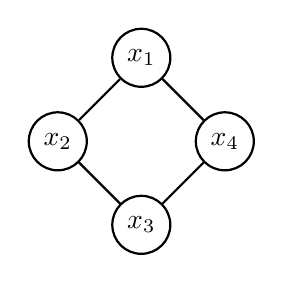
\begin{tikzpicture}[node distance={15mm}, thick, main/.style = {draw, circle}] 
            \node[main] (1) {$x_1$}; 
            \node[main] (2) [below left of=1] {$x_2$};
            \node[main] (3) [below right of=2] {$x_3$}; 
            \node[main] (4) [above right of=3] {$x_4$};
            \draw (1) -- (2);
            \draw (2) -- (3);
            \draw (4) -- (3);
            \draw (1) -- (4);
        \end{tikzpicture}
    \end{minipage}
    \hfill
    \begin{minipage}[c]{.3\linewidth} %inequalities
        \centering
        \begin{gather*}
             \begin{pmatrix}
                1 & 0.9 & ? & -0.9 \\
                0.9 & 1 & 0.9 & ? \\
                ? & 0.9 & 1 & 0.9 \\
                -0.9 & ? & 0.9 & 1
            \end{pmatrix}\\
            S^\G
        \end{gather*}
    \end{minipage}

    \caption{Example from \cite[Section 9.3]{maathuis2018handbook} of a matrix $S$ for which all completely specified submatrices of $S^\G$ are positive definite but which doesn't have a positive definite completion.}
    \label{fig-no-completion}
\end{figure}